\documentclass[10pt]{article}
\usepackage{float}
\usepackage{listings}
\usepackage{graphicx}
\usepackage{hyperref}
\usepackage{fullpage}
\begin{document}
\newenvironment{mylist}{
\begin{list}
  \setlength{\itemsep}{1pt}
  \setlength{\parskip}{0pt}
  \setlength{\parsep}{0pt}}{\end{list}
}

\lstset{language=c++}

%------------------------------------------------------------------------------
\author{N. House, K. Levner, J. Pledger, J. Ranger} 
\date{February 2nd, 2010} 
\title{System Requirements and System plan \\ \large{The K-Mapper Project V2.0}}

\maketitle
%------------------------------------------------------------------------------
\begin{abstract}
  The goal of this project is to create a tool to allow a user to draw
  Karnaugh maps of up to 6 variables.  Input can be accepted as an
  equation, truth table, Karnaugh map, or imported via a file (in pla
  form).  The application will minimize the K-Map to a minimal sum of
  products and product of sums form. The user will have the option to
  modify their input (even in a different input method than originally
  used) after obtaining output and the user may export their results
  to a file (in pla form) as well.

  This application is designed with the intended audience of
  Computer Science 2610 (Digital Systems) students. They are expected
  to have a background in KMaps, Truth Tables, and Boolean logic
  equations.

  It is intended to be run on the Linux machines found
  in the U of L computer labs. To be built, this tool will make use of
  Qt, a GUI programming library compatible with C++. It will be
  documented using Doxygen, a popular documentation tool. Both of
  these libraries are open source and come at no charge.

  The design in this document has been created with the expectation of
  future scalability concerning the number of variables, additional
  widget modification and additional input and output types. The
  design primarily focuses on encapsulation, which provides
  abstraction between the front and back end, but can still be linked
  using the adaptor design pattern. This is intended to give the user
  a great experience while still logically organizing data in the
  background.
\end{abstract}
\begin{center}
\large{\textbf{Version History}} \\

\normalsize{}
\begin{tabular}{|l|l|l|p{6cm}|}
\hline
\emph{Version} & \emph{Date}   & \emph{Author(s)} & \emph{Changes} \\
\hline\hline
1.0 & 2/2/2010 & NH, CB, JB, BK
& \begin{list}{\labelitemi}{\leftmargin=0em\topsep=0ex\itemsep=0ex}
\item{Initial version}
\end{list} \\ \hline
1.1 & 2/9/2010 & NH, CB, JB, BK 
& \begin{list}{\labelitemi}{\leftmargin=0em\topsep=0ex\itemsep=0ex}
\item{Minor grammatical corrections}
\end{list} \\ \hline
2.0 & 3/17/2010 & NH, JR, KL, JP
& \begin{list}{\labelitemi}{\leftmargin=0em\topsep=0ex\itemsep=0ex}
\item{Updated object models to reflect refactoring (See section~\ref{OMV2Changes})}
\item{Updated program screenshots}
\item{Added additional coding conventions}
\item{Fixed additional grammatical errors}
\end{list} \\ \hline 
2.1 & 3/23/2010 & NH, JR, KL, JP
& \begin{list}{\labelitemi}{\leftmargin=0em\topsep=0ex\itemsep=0ex}
\item{Added legends to activity model and object model}
\item{Updated equation input dialog screenshot}
\item{Fixed more grammatical errors}
\end{list} \\ \hline 
\end{tabular}
\end{center}
%------------------------------------------------------------------------------
\pagebreak
\tableofcontents
\pagebreak
%\twocolumn
%------------------------------------------------------------------------------
\section{Introduction}
This document intends to serve as an outline of the implementation of
the KMapper project in it's entirety.  

%------------------------------------------------------------------------------
\section{Behavioral Models}
%------------------------------------------------------------------------------
\subsection{Activity Model}
This model (fig.~\ref{activityModelFig}) represents the data flow
corresponding to the choices that the user makes. First, the user will
be prompted to select their input type. If the user chooses to input a
truth table, Equation or Karnaugh map, they will be prompted to select
how many variables they wish to use.  After submitting their input or
importing a file, the user will view the results. The user will then
have the ability to export the data to a file, modify the input, start
new input, or quit.

\begin{figure}[ht]
\caption{Activity Diagram}
\label{activityModelFig}
\centering
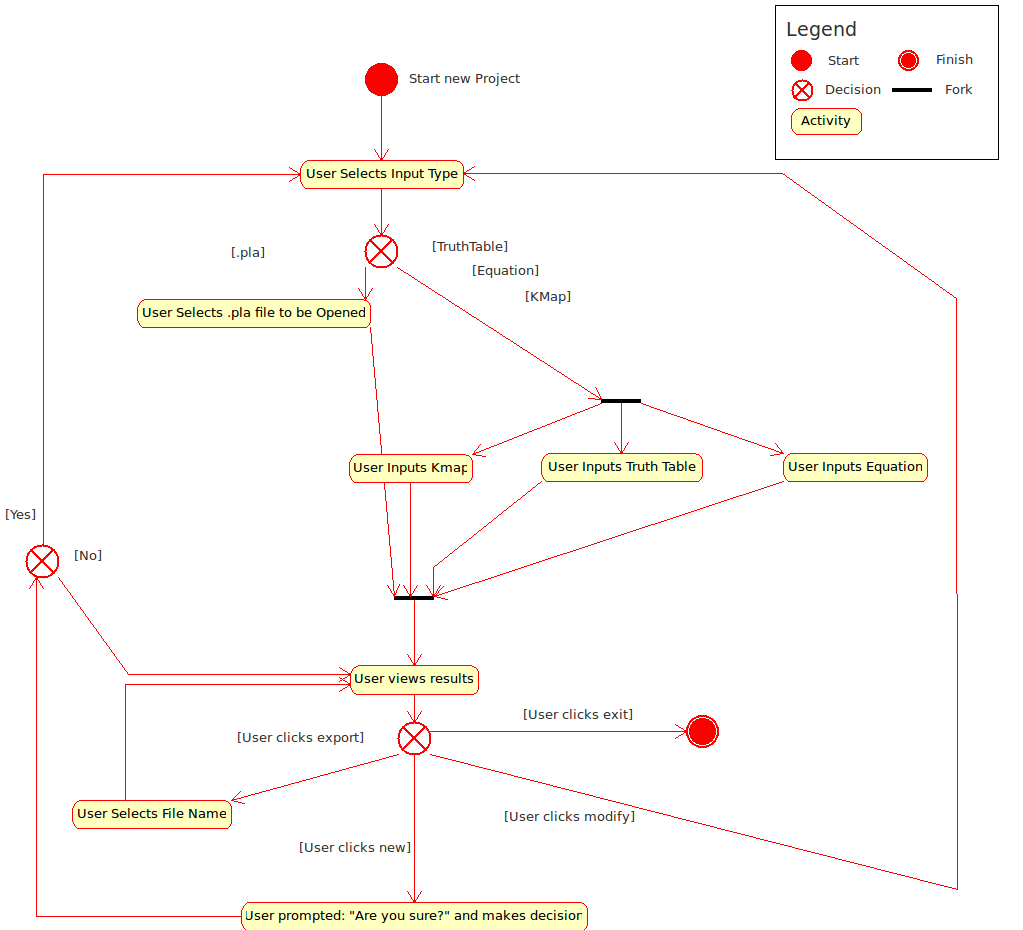
\includegraphics[width=.9\linewidth]{activityDiagram.png}
\end{figure}
%------------------------------------------------------------------------------
\subsection{State Model}
\label{stateModel}
The state model in fig.~\ref{stateModelFig} shows the different states
of the program's GUI from the user's point of view. These specific
states represent points in the program in which the user will have to
choose an action in order to move to another state. From any state,
the user may also choose to exit the program.
\begin{figure}[ht]
\caption{GUI State Model}
\label{stateModelFig}
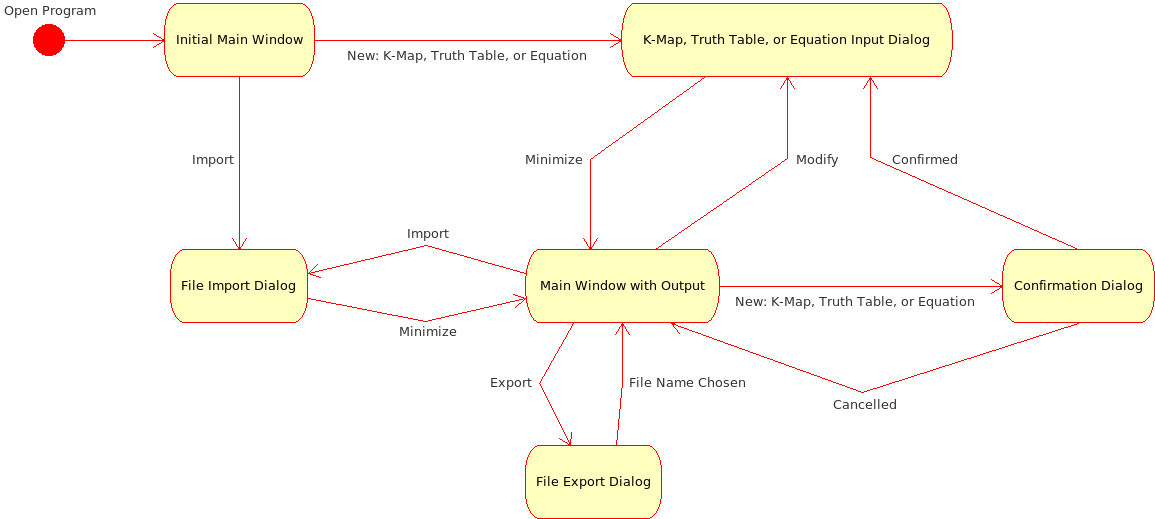
\includegraphics[width=.9\linewidth]{stateModel.png}
\end{figure}
%------------------------------------------------------------------------------
\section{Object Models}
\label{objectModels}
The object model presented here outlines the classes to be implemented
in the project, as well as some of the required inheritance from
external libraries.  

In this model, the adaptor classes provide methods to the GUI front
end to interpret data from DataBackend into the appropriate GUI
element.  It also allows communication in the opposite direction,
where elements in the graphical front end can save their data into the
back end.  All of the adaptor classes are pure virtual, that is, their
functions must be implemented by the DataBackend.  This ensures
compatibility of any future Backend representation with the current
front end.

In addition to the adaptor classes, there are two widget classes that
have been created to provide a specialized way of displaying both
truth tables and K-Maps.  These widgets will be created by either
creating a specialization of the QTable widget, or by implementing a
new widget by sub-classing QWidget.  A specialized widget for inputting
equations will probably not be necessary, as the QTextBox widget
provides sufficient functionality to input a string.

The final type of class in the model is the Dialogs, which are
sub-classed from QDialog.  These are specialized dialogs used to either
input new data to the back end, or modify the existing data.  They will
contain the appropriate type of widget, depending on the type of input
the dialog is meant to take.  It should be noted here that a
specialized dialog for file input is unnecessary, as the provided
QFileDialog is sufficient.

More detailed descriptions of the individual classes can be found in
section~\ref{classDescriptions}.
%------------------------------------------------------------------------------
\subsection{Changes In Version 2.0}
\label{OMV2Changes}
Since the first iteration of the project, the following has changed in
our object model.
\begin{itemize}
\item{TTVal class has been added to wrap the enumerated type which is
    the underlying data type of the DataBackend}
\item{Adaptor classes are now pure virtual classes, as they can only
    declare the interface that must be implemented in the DataBackend.
    This is standard for the adaptor pattern.}
\item{DataBackend now inherits from all of the adaptor classes, as it
    must implement that functionality to ensure proper function of the
    front end}
\item{Added MainWindowWidget, a class which acts as the central widget
    of the Main Window}
\item{Added InDialog class, a super class which includes the common
    functionality of all the input dialogs}
\end{itemize}
\begin{figure}[ht]
\caption{Object Model}
\label{objectModelFig}
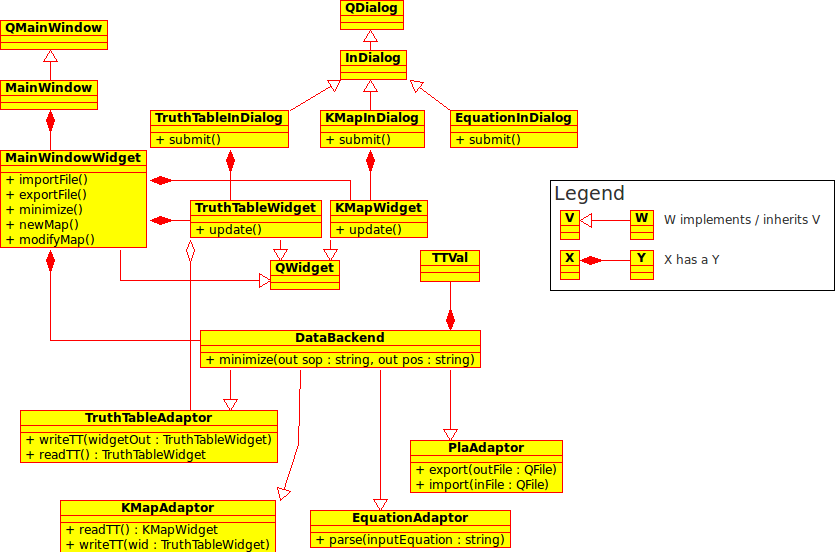
\includegraphics[width=.9\linewidth]{objectModel.png}
\end{figure}
%------------------------------------------------------------------------------
\section{Class Descriptions}
\label{classDescriptions}
These class descriptions are intended to give a introduction to the
functionality of each class, and an overview of how the classes
interact with each other.  For a graphical representation of the object
model, see figure~\ref{objectModelFig}.
%------------------------------------------------------------------------------
\subsection{DataBackend}
The DataBackend class holds all the data and implements the
Quine-McCluskey algorithm to reduce the truth table to minimal POS and
SOP form.  This class is intended to house the entirety of back end
functionality, as well as to implement any functions inherited from
the adaptor classes.
%------------------------------------------------------------------------------
\subsection{EquationAdaptor}
The EquationAdaptor class is a pure virtual class which is inherited
by DataBackend.  It provides declares a conversion method called
parse() which accepts a string, and then parses it into the common
data format inherited from DataBackend.
%------------------------------------------------------------------------------
\subsection{EquationInDialog}
EquationInDialog provides a dialog which allows users to input a
truth table in equation form.  This class uses methods from EquationAdaptor
to pass data into the back end.
%------------------------------------------------------------------------------
\subsection{InDialog}
Super class to all the other input dialogs, which provides
methods/widgets to change number of variables and variable names.
%------------------------------------------------------------------------------
\subsection{KMapAdaptor}
The KMapAdaptor class is a pure virtual class which is inherited by
DataBackend.  It provides the interface necessary for the KMapWidget
to display the data.
%------------------------------------------------------------------------------
\subsection{KMapInDialog}
The KMapInDialog provides and input dialog which allows the user to
either input a new K-Map or modify the one currently stored in the
back end, as well as change the number of variables and variable
names.  User interaction with data occurs via a KMapWidget, which in
turn writes to the back end via functions defined in KMapAdaptor.
%------------------------------------------------------------------------------
\subsection{KMapWidget}
The KMapWidget is a graphical representation of a K-Map, and is a
specialization of Qt's QTableWidget.  QTableWidget already implements
most of the functionality required, the major changes are for the
style and input methods of the widget.
%------------------------------------------------------------------------------
\subsection{MainWindow}
The MainWindow class contains the applications main interface.  It
inherits all functionality from QMainWindow, as well as providing all
the useful data display methods.  It contains a DataBackend object,
which is the central data location for the entire program.  A
graphical presentation of the main window can be found in
section~\ref{UIDesign}.
%------------------------------------------------------------------------------
\subsection{MainWindowWidget}
The MainWindowWidget acts as the central widget to the MainWindow, and
holds all widgets to be displayed on the MainWindow.
%------------------------------------------------------------------------------
\subsection{PlaAdaptor}
PlaAdaptor is another pure virtual adaptor class inherited by
DataBackend It provides file input and output through the following
two functions:
\begin{itemize}
\item{import(QFile*) - reads file specified by a QFile object and
    stores the info in the Backend}
\item{export(QFile*) - writes the content of the Backend to file
    specified by a QFile object}
\end{itemize}
This class has nothing to do with actually getting the file name from
the user, it simply opens a preselected file (possibly coming from
Qt's built in FileDialog) and either reads or writes to it.
%------------------------------------------------------------------------------
\subsection{TruthTableAdaptor}
The TruthTableAdaptor class is a pure virtual base class inherited by
DataBackend.  It provides function definitions for all accessor
methods needed for the TruthTableWidget
%------------------------------------------------------------------------------
\subsection{TruthTableInDialog}
The TruthTableInDialog provides and input dialog which allows the user
to either input a new truth table or modify the one currently stored
in the back end, as well as modify the number of variables and the
variable names.  User interaction with the data occurs via a
TruthTableWidget, which in turn writes to the back end via functions
defined in TruthTableAdaptor.
%------------------------------------------------------------------------------
\subsection{TruthTableWidget}
The TruthTableWidget is a graphical representation of a truth table, and is a
specialization of Qt's QTableWidget.  QTableWidget already implements
most of the functionality required, the major changes are for the
style and input methods of the widget.
%------------------------------------------------------------------------------
\subsection{TTVal}
TTVal is a class which contains the data type for each element in the
Truth Table.  This wrapper provides the accessor and modifier methods
needed to read, write, and minimize the truth table, such as
conversion to string, incrementing by one, and comparison.
%------------------------------------------------------------------------------
\section{UI Design}
\label{UIDesign}
\subsection{Inputting New Data}

To input new data to the program, in any format, the user uses the
``File $\rightarrow$ New'' menu (fig.~\ref{newMenuFig}).  It presents
the three possible formats (figure~\ref{inputMethodSelect}), and each
selection opens it's own specific input dialog (figures
\ref{kmapInputFig}, \ref{ttInputFig}, and \ref{eqInputFig}).

The input dialogs allow the user to select the number of variables,
the variable names, and finally input the content of the table.
Clicking ``Ok'' closes the dialog and show the updated main window.

\begin{figure}[H]
\centering
\caption{New Menu}
\label{newMenuFig}
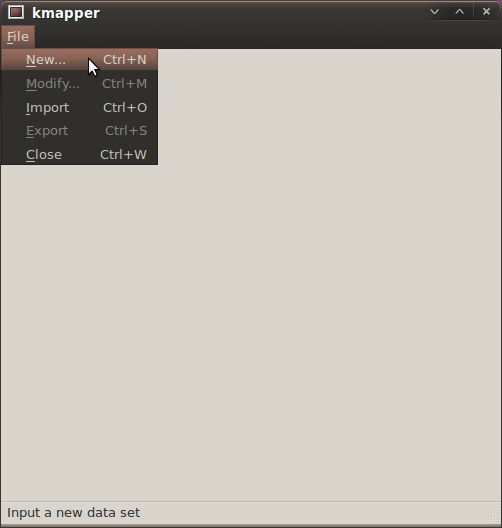
\includegraphics[width=.8\linewidth]{NewMenuExample.png}
\end{figure}

\begin{figure}[H]
\centering
\caption{Input Method Selection}
\label{inputMethodSelect}
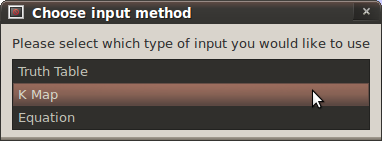
\includegraphics[width=.8\linewidth]{ChooseInputMethod.png}
\end{figure}

\begin{figure}[H]
\centering
\caption{K-Map Input Dialog}
\label{kmapInputFig}
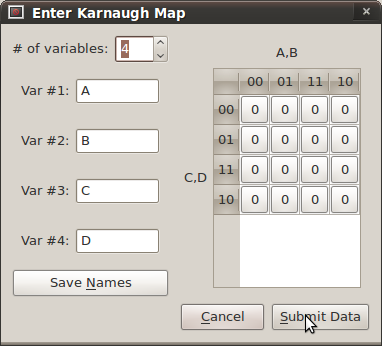
\includegraphics[width=.8\linewidth]{KmapInputExample.png}
\end{figure}

\begin{figure}[H]
\centering
\caption{Truth Table Input Dialog}
\label{ttInputFig}
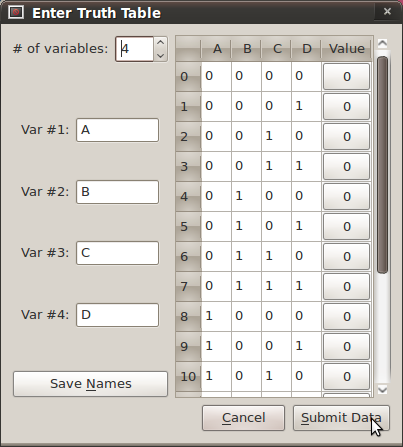
\includegraphics[width=.8\linewidth]{TtInputExample.png}
\end{figure}

\begin{figure}[H]
\centering
\caption{Equation Input Dialog}
\label{eqInputFig}
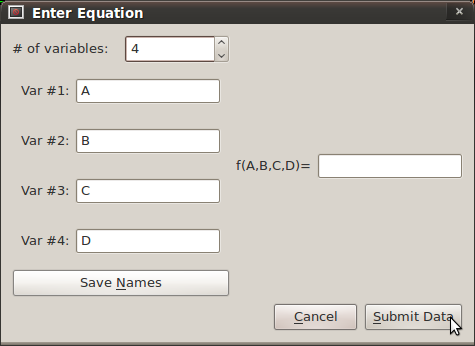
\includegraphics[width=.8\linewidth]{EquationDialogExample.png}
\end{figure}

%------------------------------------------------------------------------------
\subsection{File Operations}
Importing and exporting data to/from file is also accomplished via the
``File'' menu (fig.~\ref{importExportFig}).  Upon clicking import, the
user is presented with a file chooser dialog
(fig.~\ref{fileChooserFig}). After that the primary window will be
presented with the appropriate information loaded and the results will
be viewable (See section \ref{viewingResults}).  If the user clicks
export, the same file chooser dialog will be presented, and the
current data will be saved to the file.  If the save operation fails,
an appropriate message will be presented to the user.

\begin{figure}[H]
\centering
\caption{Import and Export Menus}
\label{importExportFig}
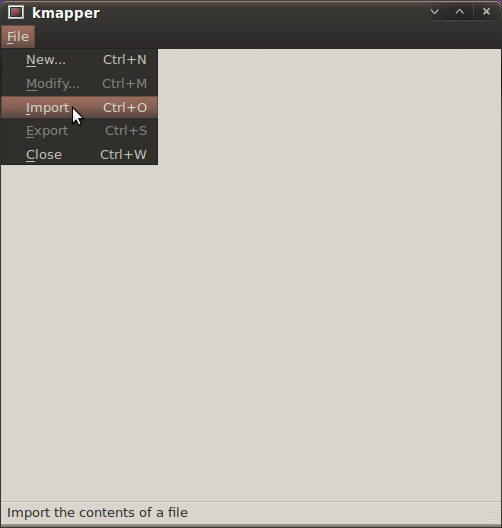
\includegraphics[width=.8\linewidth]{ImportExample.png}
\end{figure}

\begin{figure}[H]
\centering
\caption{File Chooser Dialog}
\label{fileChooserFig}
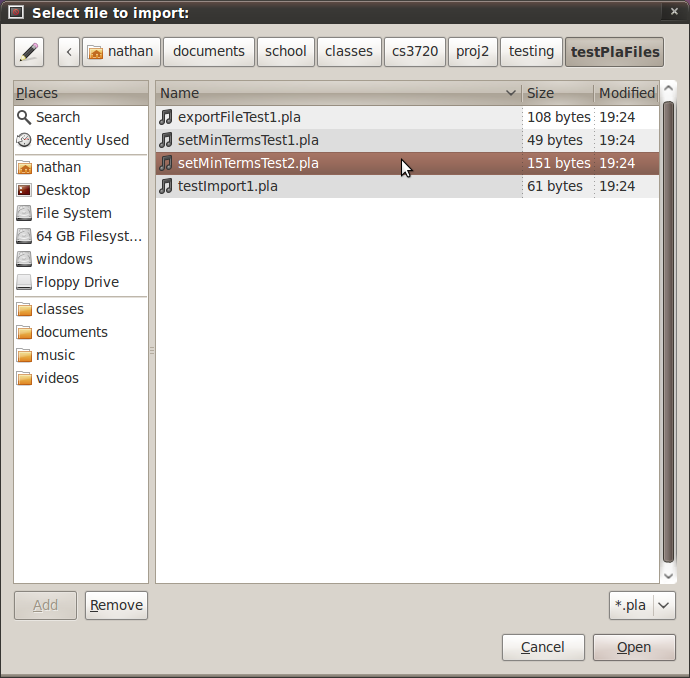
\includegraphics[width=.8\linewidth]{QFileDialog.png}
\end{figure}

%------------------------------------------------------------------------------
\subsection{Viewing Results}
\label{viewingResults}
Figure \ref{finalResultFig} show the results of minimization.  From
there the user can modify via ``File $\rightarrow$ Modify'' (see
fig.~\ref{finalResultFig2}), or export to file via ``File
$\rightarrow$ Export''

\begin{figure}[H]
\centering
\caption{View of Results}
\label{finalResultFig}
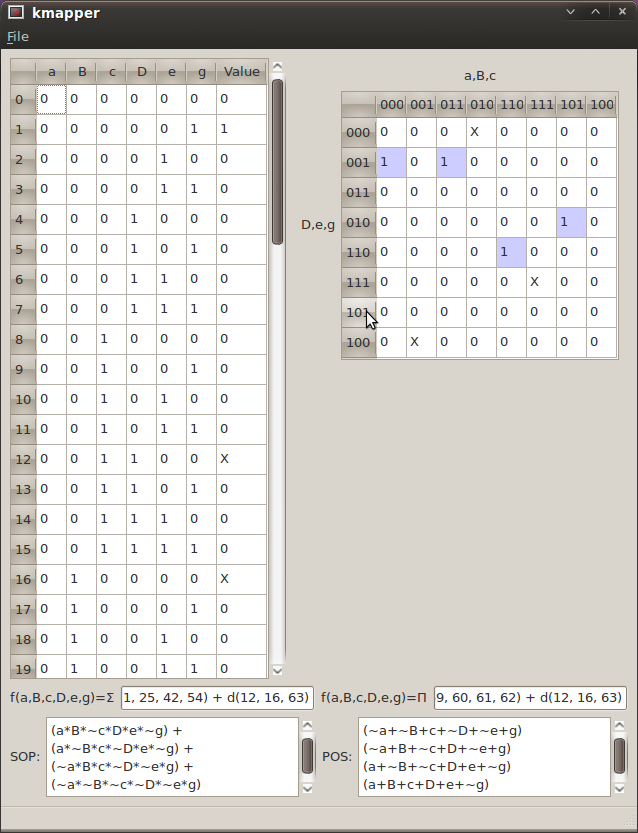
\includegraphics[width=.8\linewidth]{OutputExample1.png}
\end{figure}

\begin{figure}[H]
\centering
\caption{View of Results 2}
\label{finalResultFig2}
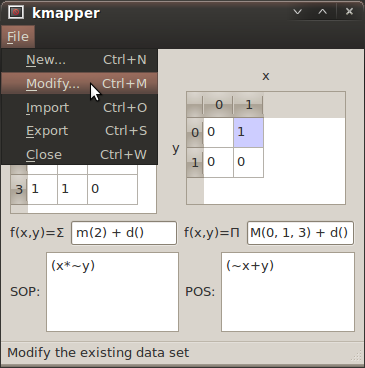
\includegraphics[width=.8\linewidth]{OutputExampleModify.png}
\end{figure}

%------------------------------------------------------------------------------
\section{Coding Standards}
%------------------------------------------------------------------------------
\subsection{Variables - Naming}
\begin{itemize}
\item{Global variables and enumerated types will be name in all
    capitals, with words separated by underscores.
    \begin{itemize}
    \item{
      \lstinline{const int MAX_NUMBER_OF_VARS=6;}
    }
    \item{
      \lstinline|enum E_TYPE{NUM=256, GRP=257};|
    }
    \end{itemize}
  }
\item{Class and Struct data types will start with a capital letter,
    and capitalize each new word.
    \begin{itemize}
    \item{
        \lstinline|class ClassExample{ ... };|
      }
    \end{itemize}
  \item{All others will be named using standard camel casing(lower
      case to start followed by capitals for each new word).
      \begin{itemize}
      \item{
          \lstinline{int thisIsAnExample;}
        }
      \item{
          \lstinline{string myName;}
        }
    
      \end{itemize}
    }}
  \end{itemize}
%-----------------------------------------------------------------------------
\subsection{Variables - Miscellaneous}
\begin{itemize}
\item{Global variables will always be declared constant.}
\item{Enumerated types will have their values manually defined and
    start at a minimum value of 256 to prevent potential conflicts
    with ASCII characters.}
\end{itemize}

%-----------------------------------------------------------------------------
\subsection{Files}
\begin{itemize}
\item{File names should be indicative of what they contain and/or
    what they do.}
\item{File names should not have spaces.}
\item{Temporary files(for file I/O) shall be used whenever loss of
    data map occur.}
\end{itemize}
%-----------------------------------------------------------------------------
\subsection{Commenting}
\begin{itemize}
\item{Comments shall follow the Doxygen coding style.
    \href{http://www.doxygen.nl/manual.html}{http://www.doxygen.nl/manual.html}}
\item{Comments for both functions and classes shall be placed directly
    above the item being described.}
\item{Brief descriptions are in header files, and should briefly
    describe what the function is doing}
\item{Long descriptions are in implementation files, and should
  briefly explain how the function will be completing it's goal}
\item{Variables should be commented in line, with the ///$<$ tag}
\item{For a sample header file, see appendix~\ref{sampleHeader}}
\end{itemize}
%----------------------------------------------------------------------------
\subsection{General}
\begin{itemize}
\item{Code revisions should compile before being submitted, if they do not:
    \begin{itemize}
    \item{Comment out the section of code changed so it will compile.}
    \item{Leave a message when committing(-m flag) stating what/where
        the error is coming from.}
    \end{itemize}
  }
\item{Commit changes before starting a new section/branch
    of coding.}
\item{If a function is returning 'placeholder data', make sure that it
    is obviously a placeholder value.
    \begin{itemize}
    \item{Using a -1 when returning an integer.}
    \end{itemize}
}
\item{Functions should be grouped in the header file in some logical way}
\item{Functions in implementation files should be in the same order as
  they appear in the header file}
\item{Sections of [repeated] similar code that can be converted to
    functions should be converted.}
\end{itemize}
%----------------------------------------------------------------------------
\clearpage
\appendix
\section{Sample Header}
\label{sampleHeader}
\lstinputlisting{../standards/interfaceFileTemplate.h}
%----------------------------------------------------------------------------
%\clearpage
%\section{Headers}
%\label{headers}
%\subsection{DataBackend.h}
\lstinputlisting{../../src/DataBackend.h}
\subsection{EquationInDialog.h}
\lstinputlisting{../../src/EquationInDialog.h}
\subsection{InDialog.h}
\lstinputlisting{../../src/InDialog.h}
\subsection{InputVariableNameWidget.h}
\lstinputlisting{../../src/InputVariableNameWidget.h}
\subsection{KMapInDialog.h}
\lstinputlisting{../../src/KMapInDialog.h}
\subsection{KMapWidget.h}
\lstinputlisting{../../src/KMapWidget.h}
\subsection{MainWindow.h}
\lstinputlisting{../../src/MainWindow.h}
\subsection{MainWindowWidget.h}
\lstinputlisting{../../src/MainWindowWidget.h}
\subsection{TruthTableInDialog.h}
\lstinputlisting{../../src/TruthTableInDialog.h}
\subsection{TruthTableWidget.h}
\lstinputlisting{../../src/TruthTableWidget.h}
\subsection{TTVal.h}
\lstinputlisting{../../src/TTVal.h}

\end{document}
